\chapter{Tworzenie i charakterystyka tras}\label{chap:charakterystyka-tras}
Tworzenie trasy polega na zapisaniu w systemie pozycji, ustalonych przy użyciu nawigacji satelitarnej, na których użytkownik znajdował się w trakcie treningu tak jak zostało to pokazane na rysunku przedstawiającym fragment utworzonej trasy \ref{image:mapka_fragment_trasy}, na którym linią ciągłą zaznaczono rzeczywistą trasę pokonaną przez biegacza, a kropkami reprezentację trasy zapisaną w systemie. Zapamiętywane są tylko te punkty, które znajdują się w odległości nie mniejszej niż 10 metrów od swojego poprzednika. Zaproponowana minimalna odległość pomiędzy punktami, pozwoli na osiągnięcie dostatecznie dokładnego przebiegu trasy, przy jednoczesnym zapobiegnięciu wystąpienia problemu, opisanego w rozdziale \ref{chap:wahania-pozycji}.

\begin{figure}[h]
\begin{center}
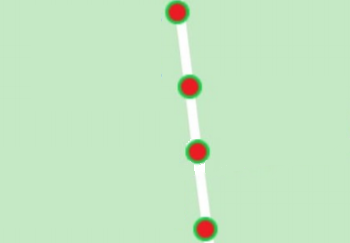
\includegraphics{img/mapka_fragment_trasy.png}
\caption{Fragment utworzonej trasy. [Opracowanie własne]}\label{image:mapka_fragment_trasy}
\end{center}
\end{figure}

Zawody biegowe w których biegacze biorą udział, różnią się trasami, na jakich są przeprowadzane. Ich dystans może wynosić od kilku do kilkudziesięciu kilometrów. Zawody odbywające się w mieście zwykle odbywają się na płaskiej nawierzchni asfaltowej, podczas gdy biegi organizowane w górach wymagają często od zawodników podbiegania pod jakiś szczyt górski lub zbiegania z niego. Nie inaczej jest z przygotowaniem do konkretnych zawodów. Chcąc jak najefektywniej przygotować się do startu, biegacz powinien trenować w warunkach zbliżonych do tych, które może spotkać na zawodach. Z tego względu aplikacja tworzona w ramach niniejszej pracy umożliwia użytkownikom wyszukiwanie tras treningowych, które spełnią ich preferencje. Niniejszy rozdział jest realizacją części pierwszego celu przedstawionego w rozdziale \ref{chap:cele-pracy}. Omówiono w nim cechy, które mogą zostać przypisane do trasy, sposób ich wyznaczenia na podstawie danych lokalizacyjnych oraz kryteria wyszukiwania używane podczas przeglądania tras. 
\section{Możliwe cechy trasy}\label{chap:opis-cech}
Do każdej trasy mogą zostać przypisane 3 cechy.
\begin{itemize}
\item{\textbf{Dystans}} - określa jak długa jest trasa. Wartość wyrażona jest w kilometrach.
\item{\textbf{Poziom terenu}} - Reprezentuje zmianę wysokości nad poziomem morza pomiędzy początkiem a końcem trasy. Wartości które może przyjąć ta cecha to:
\begin{itemize}
\item{Wyrównany} - gdy wysokość nad poziomem morze nie zmienia się lub zmienia się nieznacznie,
\item{Rosnący} - gdy wysokość nad poziomem morza wzrasta,
\item{Malejący} - gdy wysokość nad poziomem morza maleje.
\end{itemize}
\item{\textbf{Twardość nawierzchni}} - Wyraża jaka część całej trasy przebiega przez nawierzchnię utwardzoną (na przykład asfalt lub kostka brukowa) w stosunku do nawierzchni nieutwardzonej (na przykład piasek lub trawa). Wartość wyrażona jest w procentach. Przykładowo wartość 60\% dla trasy o dystansie 10 kilometrów oznacza, że 6 kilometrów prowadzi przez nawierzchnię utwardzoną, a 4 kilometry przez nieutwardzoną.
\end{itemize}
\section{Przypisanie cech do trasy}\label{chap:przypisanie-cech}
\subsection{Długość trasy}
Długość trasy przypisywana jest bezpośrednio po ukończeniu treningu. Jej wyznaczenie polega na zsumowaniu odległości pomiędzy wszystkimi następującymi po sobie punktami przy użyciu wzorów \ref{eq:haversine11},  \ref{eq:haversine2} i \ref{eq:haversine3}.

\subsection{Poziom terenu}
Określenie poziomu terenu odbywa się poprzez obliczenie różnicy wysokości nad poziomem morza pomiędzy punktem rozpoczynającym oraz kończącym trasę i przypisanie odpowiednio poziomu:
\begin{itemize}
\item{\textbf{wyrównanego}} - gdy różnica nie przekracza 10\%,
\item{\textbf{rosnącego}} - gdy wysokość punktu końcowego jest większa od wysokości punktu początkowego o więcej niż 10\%,
\item{\textbf{malejącego}} - gdy wysokość punktu początkowego jest większa od wysokości punktu końcowego o więcej niż 10\%.
\end {itemize}
Należy mieć na uwadze, że w przypadku wystąpienia problemu opisanego w rozdziale \ref{chap:problem-poziom-terenu}, cecha ta będzie musiała zostać ustalona przez użytkownika.

\subsection{Twardość nawierzchni}\label{chapter:wyznaczenie-twardosc}
W celu umożliwienia automatycznego przypisania twardość nawierzchni, posłużono się serwisem OpenStreetMap \cite{osm}. Narzędzie to pozwala scharakteryzować podłoże ustalonego przez klienta obszaru. Musi on być zdefiniowany w formie prostokąta, a odbywa się to poprzez dostarczenie serwisowi współrzędnych geograficznych jego lewej dolnej oraz prawej górnej krawędzi. Zdefiniowane przykładowego obszaru zostało pokazane na rysunku \ref{image:mapka_obszar}. Kropkami oznaczono podane współrzędne geograficzne, natomiast linia ciągła definiuje obszar, który zostanie poddany analizie. W odpowiedzi klient otrzymuje charakterystykę wszystkich dróg, które znalazły się w zdefiniowanym obszarze \cite{osm-docs-wiki}. Rodzaj nawierzchni nie jest zwracany w formie „utwardzona” bądź „nieutwardzona”, lecz w formie sprecyzowanej, na przykład „asfalt” lub „trawa”, dlatego pierwszym krokiem którego trzeba się podjąć po otrzymaniu odpowiedzi, jest przyporządkowanie etykiety  „utwardzona” bądź „nieutwardzona” dla każdego z otrzymanych obiektów. Przyporządkowanie wszystkich możliwych do otrzymania rodzajów nawierzchni zostało pokazane w tabeli \ref{table:rodzaje-nawierzchni} \cite{osm-surface}.

\begin{figure}[h]\label{fig:miary}
\begin{center}
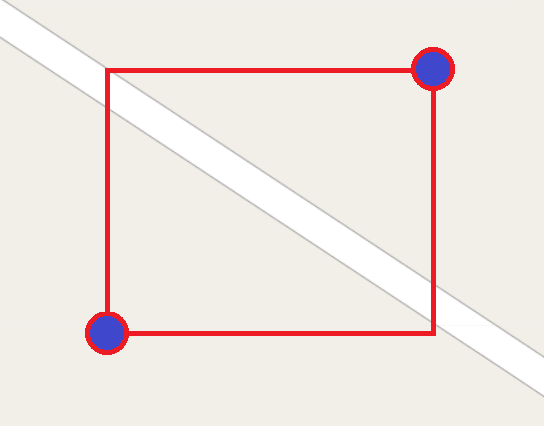
\includegraphics[width=2in]{img/mapka_obszar.png}
\caption{Obszar poddany analizie [Opracowanie własne]}\label{image:mapka_obszar}
\end{center}
\end{figure}

\begin{table}[thb]
\caption{Przyporządkowanie konkretnego rodzaju nawierzchni do jej reprezentacji w tworzonym systemie \cite{osm-surface}}.\label{table:rodzaje-nawierzchni}
\centering\renewcommand\cellalign{lc}
\setcellgapes{3pt}\makegapedcells
\begin{tabular}{|c|c|} \hline
\textbf{Nawierzchnia utwardzona} & \textbf{Nawierzchnia nieutwardzona} \\ \hline
\makecell{paved, asphalt, concrete,\\concrete:lanes, concrete:plates,\\paving\textunderscore stones, sett,\\unhewn\textunderscore cobblestone,\\cobblestone, metal, wood,\\metal\textunderscore grid } & \makecell{ unpaved, compacted, fine\textunderscore gravel,\\gravel, pebblestone, dirt,\\earth, grass, grass\textunderscore paver,\\ground, mud, sand, woodchips,\\snow, ice, salt, clay, tartan,\\artifical\textunderscore turf, decoturf, carpet} \\ \hline
\end{tabular}
\end{table}

Tworzone przez użytkowników trasy zapisywane są w formie punktów, dlatego przed skorzystaniem z serwisu OpenStreetMap, należy zdefiniować wspomniany prostokątny obszar poszukiwań. Korzystając ze wzoru \cite{eq:haversine_generowanie_punktu} wyznaczane są więc 2 nowe punkty: oddalony o 10 metrów i 225 stopni względem północy oraz oddalony o 10 metrów i 45 stopni względem północy. Po ustaleniu rodzaju nawierzchni dla każdego z punktów trasy, możliwe jest wyliczenie wartości procentowej, a tym samym określenie cechy według wzoru:
\begin{equation}\label{eq:haversine1}
{Twardosc\hspace{0.15cm} nawierzchni} = \frac{u}{u + n} \cdot 100,
\end{equation}
gdzie \(u\) oznacza liczbę obiektów z etykietą  „utwardzona”, \(n\) liczbę obiektów z etykietą  „nieutwardzona”.
Z uwagi na czytelność wynik zaokrąglany jest do liczby całkowitej.
Należy mieć na uwadze, że OpenStreetMap jest projektem tworzonym przez społeczność i dla pewnych dróg rodzaj nawierzchni mógł być przypisany błędnie bądź nie przypisany wcale. Wartość określonej cechy powinna być zatem traktowana w formie propozycji, którą użytkownik tworzący trasę może poprawić wedle własnego uznania.

\section{Kryteria wyszukiwania tras}\label{chap:kryteria}
Kryteria wyszukiwania są ściśle powiązane z cechami opisanymi w rozdziale \ref{chap:opis-cech}. Dokonano jedynie kilku usprawnień mających na celu wygodę użytkownika.
\begin{itemize}
\item{Kryterium \textbf{długości trasy} przyjmuje wartości „od” oraz „do”. Oznacza to, że lista wynikowa zawiera trasy nie krótsze niż pierwsza z nich, a jednocześnie nie dłuższe niż druga z nich. Największa wartość, którą można określić wynosi 20 kilometrów.  Po jej przekroczeniu, przy wyszukiwaniu pod uwagę brane są trasy o nieograniczonej maksymalnej długości,}
\item{Przy filtrowaniu ze względu na \textbf{poziom terenu} oprócz konkretnych wartości cechy możliwe jest także wybranie opcji „każdy”. Oznacza to, że trasy nie będą filtrowane według tej cechy.}
\item{\textbf{Twardość nawierzchni} podobnie jak w przypadku długości trasy określana jest jako zakres  „od, do”. Wartość maksymalna wynosi 100\%.}
\end{itemize}
Oprócz tego użytkownik musi określić maksymalny promień wyszukiwania względem jego obecnej lokalizacji. Dzięki temu jest on świadomy, że zostały mu pokazane wszystkie trasy z interesującego go obszaru. Nie bez znaczenia jest także fakt, że zapobiegnie to pobieraniu z bazy danych wszystkich istniejących tras, co miałoby znaczący wpływ na wykorzystanie łącza oraz wydajność zarówno aplikacji serwerowej jak i aplikacji mobilnej.